\chapter{Chapter 1: Oscillations}
\section{Simple Harmonic Motion}
\subsection*{Mass on a Spring}
Consider a mass $m$ laying on a frictionless flat plane attached to some spring with spring constant $k$. If the spring is at equilibrium at $x=0$ and the mass is given some small displacement $x_0$ and initial velocity $\dot x_0$, find the equations of motion.

The force the spring exerts on the mass, the \textit{restoring force}, is described by Hooke's Law:
\[ F = -kx \]
and Newton's Second Law gives us the differential equation $m\ddot x = - kx $ (where $\dot x$ denotes the first derivative of $x$ with respect to $t$, and $\ddot x$ denotes the second derivtaive), that has the initial condition $x(0) = x_0$ and $\dot x(0) = \dot x_0$.

To search for a solution to this, we search for a function where its second derivative is proportional to the negative of itself. The familiar family of functions which we know to follow this rule are the sinusoidal functions--$\sin x$ and $\cos x$. 

In particular, if $x_1(t) = a_1\cos(b_1t)$ where $a_1$ and $b_1$ are arbitrary, we have $\ddot x_1 = -a_1b_1^2\cos(b_1t) - b_1^2x_1$. The relationship $\ddot x_1 = -b_1^2x_1$ is exactly identical to our Newton's Second Law equation if $b_1^2 = k/m$, so the function $x_1(t) = a_1\cos(\sqrt{k/m} \, t)$ describes the motion of the mass on the spring. On the other hand, if we consider a function of the form $x_2(t) = a_2\sin(b_2t)$, the exact same process leads us to the solution $x_2(t) = a_2\sin(\sqrt{k/m}\, t)$.

The values $a_1$ and $a_2$ that determine the exact solution are found by the analyzing the initial conditions. However, we will find that not all types of movement can be described by $x_1$ or $x_2$ individually. For example, if $x_0 = 0$ and $\dot x_0 = 5$, it is \textit{impossible} for the movement to be described by $x_1(t)$, no matter how we choose $a_1$. To remedy this, we will note the fact that any second order linear differential equation has two linearly independent solutions, and the solution for any set of initial values can be given by the superposition (sum) of these solutions \textit{(See a text on differential equations for more detail in where this theorem comes from and how it is proven)}.

Therefore, the solution to the differential equation $m\ddot x + kx = 0$, in the most generality possible, is given by
\[ x(t) = A\cos\pqty{\sqrt{\frac{k}{m}}t} + B\sin\pqty{\sqrt{\frac{k}{m}}t}\]
If we define a quantity called the \textit{angular frequency} $\omega\equiv \sqrt{k/m}$, the equation of motion becomes $\ddot x + \omega^2 x = 0$ and the solution is
\[ x(t) = A\cos(\omega t) + B\sin(\omega t) \]
This gives $x(0) = x_0 = A$ and $\dot x(0) = \dot x_0 = B\omega$, which allows us to solve for the values of $A$ and $B$ to find
\begin{equation}\label{superpos}
    x(t) = x_0\cos(\omega t) + \frac{\dot x_0}{\omega }\sin(\omega t)
\end{equation}
This is a periodic function, so if the period is given by $T$, we have
\[ \cos(\omega(t + T)) = \cos(\omega t) \]
with an analogous equation for $\sin$. This implies $\omega (t + T) = \omega t + 2\pi$, so $T = 2\pi/\omega$.

We also define a quantity $\nu = 1/T$, called the \textit{frequency}. This represents the number of revolutions per second.

Using trigonometric properties, we may also write
\[ x(t) = A\cos(\omega t + \phi) \]
where $A$ is the amplitude and $\phi$ is a quantity known as the \textbf{phase shift}. Finding the amplitude for a given initial velocity and position is a simple exercise in the conservation of energy. The kinetic energy of the mass is given by $K = \frac{1}{2}m\dot x^2$ and the potential energy stored in the spring is given by $U = \frac{1}{2}kx^2$. As there are no nonconservative forces acting on the system, we know that the total mechanical energy $E\equiv K+U = \frac{1}{2}m\dot x^2 + \frac{1}{2}kx^2$ is constant. 

At the amplitude points $x=\pm A$ (when the mass switches direction), the object is momentarily at rest so the kinetic energy is zero. Thus, all of the energy in the system is stored in the spring, so $E = \frac{1}{2}kA^2$. With the conservation of energy, we can find a relationship between the position $x(t)$ and velocity $\dot x(t)$ with
\[ \frac{1}{2}kA^2 = \frac{1}{2}k\bqty{x(t)}^2 + \frac{1}{2}m\bqty{\dot x(t)}^2\]
In particular, at $t=0$,
\[ \frac{1}{2}kA^2 = \frac{1}{2}kx_0^2 + \frac{1}{2}m\dot x_0^2 \]
which can be solved for the amplitude $A$:
\begin{align}
    A &= \sqrt{x_0^2 + \frac{m}{k}\dot x_0^2} \nonumber \\
    &= \sqrt{x_0^2 + \frac{\dot x_0^2}{\omega^2}}
\end{align}
the phase shift can also be obtained by noting that
\[ A\cos(\phi) = x_0 \quad\text{and}\quad -A\omega\sin(\phi) = \dot x_0\]
and solving simultaneously. One special case to be aware of is that if $\dot x_0 =0$--that is, if we release the object from rest--we find $A = x_0$ and $\phi = 0$, so the equation of motion is simply
\[ x(t) = x_0\cos(\omega t) \]
A similar, yet less common case is when $x_0 = 0$. This corresponds to when we release the object from equilibrium with an initial velocity. In this case, we find $A = \dot x_0/\omega$ and $\phi = -\pi/2$, so
\[ x(t) = \frac{\dot x_0}{\omega}\cos(\omega t - \pi/2) = \frac{\dot x_0}{\omega}\sin(\omega t)\]
We may notice that the two equations we found for $x_0 = 0$ and $\dot x_0 = 0$ are exactly the two linearly independent solutions that comprise (\ref{superpos}). This tells us that we can understand the $\cos$ term as representing the contribution from the initial position/initial potential energy, and the $\sin$ term as representing the contribution from the initial velocity/initial kinetic energy.

We can represent the potential and kinetic energies as functions of $t$ by simply plugging in $x(t)$ and $\dot x(t)$ to find
\begin{align}
    K &= \frac{1}{2}m\dot x^2 \nonumber \\ 
    &= \frac{1}{2}m\omega^2 A^2\sin^2(\omega t + \phi)   \\
    U &= \frac{1}{2}kx^2 \nonumber \\
    &= \frac{1}{2}kA^2\cos^2(\omega t+\phi) \nonumber \\
    &= \frac{1}{2}m\omega^2A^2\cos^2(\omega t + \phi) \quad\quad(\text{plugging in } k = m\omega^2 )
\end{align}
One important fact is that $T$ and $V$ are perfectly out of phase with each other, so when one is at a maximum, the other is at a minimum (zero in this case). We can also notice that the sum $E = U +K$ is constant at $E = \frac{1}{2}m\omega^2A^2 = \frac{1}{2}kA^2$, as we expect.
\subsection*{Simple Pendulum}
Consider a pendulum of length $\ell$ swinging on a massless, frictionless string that forms an angle $\varphi$ with the vertical. 

One way to analyze the motion of this pendulum is by considering its energy. The kinetic energy is given by $K = \frac{1}{2}mv^2 = \frac{1}{2}m\ell^2\dot \varphi^2$, and the potential energy (with $U = 0$ when the pendulum points down) is $U = mg\ell(1 - \cos\varphi)$. The total energy is their sum,
\[ E = K+U = \frac{1}{2}m\ell\pqty{\ell\dot\varphi^2 + 2g(1-\cos\varphi)}\]
Using the small-angle approximation $\cos\varphi \approx 1- \varphi^2/2$, we get
\[ E = \frac{1}{2}m\ell(\ell \dot\varphi^2 + g\varphi^2)\]
Because the energy is conserved, we know $\ell\dot\varphi^2 + g\varphi^2$ is constant, or
\[ \dv{t} (\ell\dot\varphi^2 + g\varphi^2) = 2\ell \dot\varphi\ddot \varphi + 2g\varphi\dot\varphi = 0\]
This simplifies to $\ell\ddot\varphi = -g\varphi$, which is exactly the equation for simple harmonic motion with angular frequency $\omega = \sqrt{g/\ell}$.
\subsection*{Physical Pendulum}
Consider a pendulum that forms an arbitrary shape with a center of mass that rests at a distance $\overline r$ from the origin, with a moment of inertia $I$. To find the total kinetic energy $K$, we must sum the kinetic energies of each infinitesimal particle forming the physical pendulum:
\begin{align*}
    K &= \frac{1}{2}\sum m_iv_i^2 = \frac{1}{2}\sum m_i r_i^2\dot\varphi^2 \\
    &= \frac{1}{2}\dot\varphi^2\sum m_ir_i^2 = \frac{1}{2}I\dot\varphi^2
\end{align*}
For the potential energy, we treat the pendulum as a point particle at its center of mass. That is,
\[ U = mg\overline r(1-\varphi) \approx \frac{1}{2}mg\overline r \varphi^2\]
The total mechanical energy $T+V$ is given by
\[ E = K+U = \frac{1}{2}\pqty{I\dot\varphi^2 + mg\overline r\varphi^2}\]
Since energy is conserved, $\dot E = 0$ so
\begin{align*}
    \dot E &= I\dot\varphi \ddot\varphi + mg\overline r \varphi\dot\varphi \\
    &= I\ddot \varphi + mg\overline r \varphi = 0
\end{align*}
This gives the equation of motion
\[ \ddot\varphi = -\frac{mg\overline r}{I}\varphi \]
which describes a simple harmonic oscillator with angular frequency $\omega = \sqrt{mg\overline r/I}$.
\section{Damped Harmonic Motion}
Oftentimes the motion of a spring is not perfectly harmonic, and instead decays based on its speed, giving the equation of motion
\[ m\ddot x= -kx - b\dot x\]
We define the quantity $\gamma \equiv b/m$ as the \textbf{damping constant} for the spring, and $\omega_0 \equiv \sqrt{k/m}$ as the \textbf{natural frequency} of the spring. With these constants, the equation of motion becomes  
\[ \ddot x + \gamma \dot x + \omega_0^2 x = 0\]
The motion has a characteristic equation given by $r^2 + \gamma r + \omega_0^2 = 0$. Based on the sign of the discriminant $\gamma^2 -4 \omega_0^2$, the motion may fall into one of three categories.

\begin{enumerate}
    \item \textbf{(Two Real Roots} $\gamma > 2\omega_0$\textbf{)}: We obtain the general solution $x(t) = c_1e^{r_1t} + c_2e^{r_2t}$. The roots are given by 
    \[ r_{1,2} = \frac{-\gamma \pm \sqrt{4\gamma ^2-4\omega_0^2}}{2} = -\frac{\gamma}{2} \pm \sqrt{\frac{1}{4}\gamma^2-\omega_0^2} \]
    which are easily observed to both be negative, ensuring that our solution decays over time, as expected. This corresponds to a graph that doesn't even complete one oscillation before dying off, which matches with our intuition; the discriminant is positive when $\gamma$ is very large compared to $\omega_0$, meaning that a lot of damping is happening. This type of solution is known as \textbf{overdamping}.

    We define the quantities $\mu_1 = -r_1$ and $\mu_2 = -r_2$, so the general solution takes the nice form of
    \[ x(t) = c_1e^{-\mu_1 t} + c_2e^{-\mu_2 t} \]
    Considering the case where $\gamma$ is much larger than $2\omega_0$, we can rewrite our $\mu$s as
    \[ \mu_{1,2} = \frac{\gamma}{2} \pm\frac{\gamma}{2}\sqrt{1 - \frac{4\omega_0^2}{\gamma^2}}\]
    We can expand the second term with a Taylor Series to obtain
    \[ \mu_{1,2} \approx\frac{\gamma}{2} \pm \frac{\gamma}{2}\pqty{1 - \frac{2\omega_0^2}{\gamma^2}}\]
    Where higher order terms are negligible because $4\omega_0^2/\gamma^2$ is close to zero. Then,
    \begin{align*}
        \mu_{1,2} &\approx \frac{1}{2}(\gamma\pm \gamma)  - \frac{\omega_0^2}{\gamma}
    \end{align*}
    A small amount of divergence in our approximations happens here. For $\mu_1$, the $\omega_0^2/\gamma$ term is negligible compared to $\gamma$, so we get $\mu_1 \approx \gamma$.

    For $\mu_2$, the $\omega_0^2/\gamma$ term is \textit{not} negligible compared to zero, so we get $\mu_2 \approx \omega_0^2/\gamma$. Therefore, the equation of motion becomes
    \[ x(t)\approx c_1e^{-\gamma t} + c_2e^{-(\omega_0^2/\gamma) t}\]
    Because the $c_1$ term dissipates much quicker than the $c_2$ term, as $\gamma \gg \omega_0^2/\gamma$, the motion will quickly be dominated by the $c_2$ term. 
    \item \textbf{(Two Imaginary Roots $\gamma < 2\omega_0$ }\textbf{)}: We obtain the general solution $x(t) = e^{\alpha t}\pqty{c_1 \cos (\beta t) + c_2\sin(\beta t)}$, where 
    \[ \alpha = -\gamma/2  \quad\text{and}\quad \beta = \sqrt{\omega_0^2 - \gamma^2}\]
    Further, we define the quantity $\omega_u \equiv \sqrt{\omega_0^2 - \frac{1}{4}\gamma^2}$ as the \textbf{underdamped frequency} of the oscillations, allowing us to rephrase the general solution as $x(t) = e^{-\gamma t/2}\pqty{c_1\cos(\omega_u t) + c_2\sin(\omega_u t)} = A_0e^{-\gamma t/2}\cos(\omega_u t + \phi)$. The general solution corresponds to a graph that oscillates with decreasing amplitude; this behavior is known as \textbf{underdamping}.
    \item \textbf{(Repeated Real Root} $\gamma = 2\omega_0$\textbf{)}: Finally, at the boundary between underdamping and overdamping lies \textbf{critical damping}, when $\gamma = 2\omega_0$. We find the general solution
    \[ x(t) = c_1 e^{-\gamma t/2} + c_2te^{-\gamma t/2} = c_1e^{-\omega_0t}+c_2te^{-\omega_0 t}\]
    It is not immediately obvious why the $c_2$ term is a solution to the differential equation. To show this, we will take the seemingly odd step to look back at our overdamping solution, and rewrite it as
    \[ x(t) = e^{-\mu_1 t}\pqty{c_1 + c_2e^{-(\mu_2-\mu_1)t} }\]
    And take the limit as $\mu_2-\mu_1 \to 0$. We will do a Taylor Expansion on the right term to write
    \begin{align*}
        x(t) &= e^{-\mu_1 t}\pqty{c_1 + c_2\pqty{1 - (\mu_2-\mu_1)t + \mathcal{O}((\mu_2-\mu_1)^2)}} \\
        &\approx e^{-\mu_1 t}\pqty{c_1 + c_2 -c_2(\mu_2- \mu_1)t} \\
        &= c_1e^{-\mu_1 t} + \beta te^{-\mu_1 t}
    \end{align*}
    where $\beta = c_2 - c_2(\mu_2-\mu_1)$. As $\mu_2-\mu_1 \to 0$, $\beta \to c_2$ and so we get the two independent solutions $c_1e^{-\mu_1 t} $ and $c_2te^{-\mu_1 t}$, as desired. 
\end{enumerate}
Considering the energy of the motion, we say that the total energy at a time $t$ is proportional the amplitude at that time. For underdamped motion, the motion is governed by $x(t) = A_0e^{-\gamma t/2}\cos(\omega_u t + \phi)$, and so the amplitude of oscillation at any given time is $A = A_0e^{-\gamma t/2 }$,  which tells us the total energy is given by $E = \frac{1}{2}kA^2 = \frac{1}{2}A_0ke^{-\gamma t}$. 

We also define the decay time as $\tau = 1/\gamma$, which represents the amount of time it takes for the energy to decrease by a factor of $1/e$. 

And we also define the quantity $Q \equiv \omega_0/\gamma$ as the \textbf{quality factor}, which can be thought of as representing the speed of the damping relative to the natural frequency of the system. As $Q\to\infty$, the the system approaches perfect harmonic motion and it will store energy for a long time. As $Q$ decreases, the speed of the damping increases and it will store energy for less time. 
\subsection*{Summary}
The equation of motion of a damped oscillator is given by $m\ddot x + b \dot x + kx = 0$, which has three unique families of solitions describing three different types of motion:
\begin{enumerate}
    \item $(\gamma < 2\omega_0)$; Underdamped Motion. $x(t) = ce^{-\gamma t/2}\cos(\omega_u t+\varphi)$. 
    \item $(\gamma > 2\omega_0)$; Overdamped Motion. $x(t) = c_1e^{-\mu_1 t} + c_2e^{-\mu_2 t}$.
    \item $(\gamma = 2\omega_0)$; Critically Damped Motion. $x(t) = c_1e^{-\gamma t/2} + c_2te^{-\gamma t/2}$.
\end{enumerate}
\subsection*{Electric Circuits}
The movement of charge in an $LC$ circuit is analogous to that of an undamped spring oscillator. Suppose we have a circuit with an inductor of inductance $L$ and a capacitor of capacitance $C$. Kirchoff's loop rule tells us that
\[ L\ddot Q + \frac{1}{C} Q = 0\]
Which we know to be the equation of motion for a harmonic oscillator of frequency $\omega_0 = \sqrt{1/(LC)}$, solved by
\[ Q(t) = Q_0\cos(\omega_0 t + \varphi)\]
$L$ is analogous to the mass, which is understandable because inductors tend to resist changes in current, just like mass tends to resist changes in velocity. The quantity $1/C$ is analogous to the spring constant, because a large capacitance means that more charge (analogous to amplitude) can be stored at a lower voltage (analogous to energy).

Similarly, an $LRC$ circuit is analogous to a damped spring oscillator, with the equation of motion
\[ L\ddot Q + R\dot Q + \frac{1}{C}Q = 0\]
All of the same analysis that applied to the traditional damped spring-mass oscillator applies to the circuit with resistance.
\section{Driven Harmonic Motion}
Consider a mass $m$ attached to a spring with spring constant $k$ that undergoes a damping force given by $F_\text{damping} = -b\dot x$ and is driven by some force $F_\text{driving}(t) = F_d  \cos\omega t$. It is important to note that in general, the frequency of the driving force $\omega$ is equal to neither the underdamped frequency $\omega_u$ nor the natural frequency $\omega_0$.

A sinusoidal driving force may seem like an oddly specific class of functions to limit ourselves to, but it turns out that (as we will see when we study Fourier analysis) it is actually a rather generalizable result.

The differential equation governing the motion of the damped, driven oscillator is given by
\begin{align}
    F_\text{spring} + F_\text{damping} + F_\text{driving} &= ma \nonumber \\
    \implies m\ddot x + b\dot x + kx &= F_d\cos\omega t \label{unfixed}
\end{align}
We will rewrite this as
\begin{equation} \label{realversion}
    \ddot x + \gamma \dot x + \omega_0^2x=(F_d/m)\cos\omega t
\end{equation}
where $\gamma$ and $\omega_0$ are defined as usual.

This equation is also linear, which turns out to be a pretty important realization. Suppose momentarily that we had a system with two separate driving forces $F_1(t)$ and $F_2(t)$ acting on it. If $x_1(t)$ solves $\ddot x_1 + \gamma \dot x_1 + \omega_0^2x_1 = F_1/m$ and $x_2(t)$ solves $\ddot x_2 + \gamma \dot x_2 + \omega_0^2x_2 = F_2/m$, then their sum $x_1(t) + x_2(t)$ gives
\begin{align*}
    &\dv[2]{t}(x_1 + x_2) + \gamma\dv{t}(x_1+x_2) + \omega_0^2(x_1+x_2) \\
    &= (\ddot x_1 + \gamma \dot x_1 + \omega_0^2x_1) + (\ddot x_2 +  \gamma\dot x_2 + \omega_0^2x_2) = (F_1+F_2)/m
\end{align*}
In other words, $x_1+x_2$ is a solution for the force $F_1+F_2$. This generalized quite well to any number of forces, and even an infinite number of forces.

Now, let's attempt to solve this system.
\subsection*{Solving the Differential Equation}
First, consider the equation 
\begin{equation} \label{imaginaryversion}
    \ddot y + \gamma\dot y + \omega_0^2y = (F_d/m)e^{i\omega t}
\end{equation}
This equation is not exactly physical because the driving ``force" is complex. However, we will see shortly that if we take the real component $\Re y$, we get a correct solution to the physical system. To see why this is allowed, write $y(t) = \alpha(t) + i\beta(t)$. Then, plugging $y$ into our differential equation,
\begin{align*}
    \ddot y + \gamma \dot y + \omega_0^2y &= (\ddot \alpha+\gamma\dot \alpha+\omega_0^2\alpha)+i(\ddot \beta+\gamma\dot\beta + \omega_0^2\beta) 
\end{align*}
Equating the real components, we find
\begin{align*}
    \ddot \alpha + \gamma\dot\alpha+\omega_0^2\alpha = \Re (F_d/m)e^{i\omega t} = (F_d/m)\cos(\omega t)
\end{align*}
Thus if $y$ is a solution to (\ref{imaginaryversion}), then $\Re y$ is a solution to (\ref{realversion}).

Now, to solve (\ref{imaginaryversion}), we make use of an important theorem from differential equations. For a system of the form $\sum_i a_ix^{(i)} = f(t)$, the general solution is given by the superposition of the general solution to the homogeneous version $\sum_i a_ix^{(i)} = 0$ and any solution to $\sum_i a_ix^{(i)} = f(t)$. 

Therefore, the general solution here is given by
\[ x(t) = x_\text{tr}(t) + x_\text{st}(t) \]
where $x_\text{tr}$ refers to the \textbf{transient solution} (the solution to the homogeneous system) and $x_\text{st}$ refers to the \textbf{steady state solution} (the solution caused by the driving force). As we know, for an underdamped system, we have
\[ x_\text{tr}(t) = A_\text{tr}e^{-\gamma t/2} \cos(\omega_ut + \phi_u)\]
As we can see, the amplitude of this solution dies down according to $x\propto e^{-\gamma t/2}$. We will explore how the transient solution affects the motion later, but for now we will assume that enough time has passed so that the effect of $x_\text{tr}$ is negligible, and $x\approx x_\text{st}$.

To find the steady state solution, we guess a solution of the form $y(t) = Ce^{i\omega t}$, which gives
\begin{align*}
    Ce^{i\omega t}(-\omega^2 + i\gamma \omega + \omega_0^2) = (F_d/m)e^{i\omega t}
\end{align*}
Which tells us
\[ C = \frac{F_d}{m}\frac{1}{(\omega_0^2-\omega^2)+i\gamma\omega}\]
We wish to remove the complex part from the denominator of $C$, so we multiply the numerator and the denominator by the complex conjugate of the denominator, giving
\begin{align*}
    C &= \frac{F_d}{m}\frac{(\omega_0^2-\omega^2)-i\gamma\omega}{(\omega_0^2-\omega ^2)^2+(\gamma\omega)^2}
\end{align*}
Note that $x_\text{st}(t) = \Re(Ce^{i\omega t})$ is \textbf{NOT} the same as $\Re(C)\Re(e^{i\omega t})$. Instead, we will write $C = Ae^{i\phi}$ where $A$ is real and get $x_\text{st}(t) = A\Re (e^{i\phi}e^{i\omega t})$. To do this, note that $A = \sqrt{CC^*}$, so
\begin{align*}
    A = \sqrt{CC^*} &= \sqrt{\frac{F_d^2}{m^2}\frac{[(\omega_0-\omega)^2-i\gamma\omega][(\omega_0-\omega)^2+i\gamma\omega]}{[(\omega_0^2-\omega^2)^2+(\gamma\omega)^2]^2}} \\
    &= \frac{F_d}{m}\sqrt{\frac{(\omega_0^2-\omega^2)^2+(\gamma\omega)^2}{[(\omega_0^2-\omega^2)^2+(\gamma\omega)^2]^2}} \\
    &= \frac{F_d}{m} \frac{1}{\sqrt{(\omega_0^2-\omega^2)^2+(\gamma\omega)^2}}
\end{align*}
And $\phi = \arctan(\Im C/\Re C)$, so
\begin{align*}
    \phi &= \arctan\pqty{\frac{-\gamma\omega}{\omega_0^2-\omega^2}}
\end{align*}
thus our solution becomes $x_\text{st}(t) = A\Re(e^{i\phi}e^{i\omega t}) = A\cos(\omega t + \phi)$.

The general solution is then
\begin{equation}
    x(t) = A_\text{tr}e^{-\gamma t/2}\cos(\omega_ut+\phi_u) + A\cos(\omega t+\phi)
\end{equation}
It is worth taking a second to put all of the parameters in this equation in one place:
\begin{enumerate}
    \item $A_\text{tr}$ and $\phi_u$ determine the transient motion, and are determined by the initial conditions.
    \item $\omega_u = \sqrt{\omega_0^2-\gamma^2/4}$ is the underdamped frequency.
    \item $\omega$ is the driving frequency, which is chosen arbitrarily.
    \item $A$ and $\phi$ are functions of the physical properties of the system and the properties of the driving force ($\omega$, $\gamma$, $\omega_0$, $F_d$, and $m$).
\end{enumerate}
\section{Special Cases for Frequency}
For the following cases, we assume that the transient solution has died out and we only focus on the steady state.
\subsection*{Slow Driving}
Slow driving occurs when $\omega \ll \omega_0$. In this case, we have $\phi \approx 0$ and 
\[ A \approx \frac{F_d}{m\omega_0^2} = \frac{F_d}{k}\]
Therefore $x(t)$ takes the relatively simple form
\[ x(t) = \frac{F_d}{k}\cos(\omega t)\]
Note that in this case, the spring force is given by $F_\text{spring} = -kx = -F_d\cos(\omega t)$, which is exactly equal to $-F_\text{driving}$. This makes sense; the small frequency $\omega$ implies that the object is hardly moving (and, more relevantly, hardly accelerating). This implies that the net force must be approximately zero. The damping force is more or less irrelevant because of the relatively small speed of the mass, so the damping force must more or less balance out with the spring force. 

We can also get to this conclusion by noticing that the first two terms in the $F=ma$ equation are negligible:
\[ \cancelto{\approx 0}{\ddot x + \gamma \dot x} \;\;\;\;\;\;\; + \omega_0^2x = (F_d/m)\cos\omega t\]
so $x \approx (F_d/m\omega_0^2)\cos\omega t = (F_d/k)\cos\omega t$.

To justify the $\phi\approx 0$ result, notice that the equation $F_\text{spring} = -F_\text{driving}$ tells us that the driving force (which has no phase shift) is roughly in phase with the position.
\subsection*{Fast Driving}
Fast driving occurs when $\omega \gg \omega_0$. In this case, we have $\phi = -\pi$ and $A\approx (F_d/m)(1/\sqrt{\omega^4+(\gamma\omega)^2}$. If we additionally assume $\gamma \ll \omega$, we get $A\approx F_d/(m\omega^2)$. Therefore, the position takes the form
\[ x(t) = \frac{F_d}{m\omega^2}\cos(\omega t-\pi) = -\frac{F_d}{m\omega^2}\cos(\omega t)\]
Note that the mass times acceleration is then $m\ddot x = F_d\cos\omega t$, which is exactly the driving force. In other words, the acceleration of the motion is essentially solely given by the driving force. Since we are assuming that $\omega_0 \ll \omega$ and $\gamma \ll \omega$, the spring term and the damping term are negligible compared to the driving term.
\[ \ddot x + \cancelto{\approx 0}{\gamma\dot x + \omega_0^2x} \;\;\;\; = (F_d/m)\cos\omega t\]
The $\phi\approx-\pi$ result can be understood as follows: since the driving force accounts for practically all of the motion, it must be roughly in phase with the acceleration and thus out of phase with the position.
\subsection*{Resonance}
If $\omega=\omega_0$, then we can once again simplify the expressions for $\phi$ and $A$. No restrictions need to be placed on $\gamma$, except that it must be nonzero. In this case, we find
\[ \phi = -\pi/2 \quad\text{and}\quad A= \frac{F_d}{\gamma m\omega}\]
Therefore, the position takes the form
\begin{align*}
    x(t) &= \frac{F_d}{\gamma m\omega}\cos(\omega t-\pi/2) = \frac{F_d}{\gamma m\omega}\sin(\omega t)
\end{align*}
Note that the damping force is then $F_\text{damping} = -(\gamma m)\dot x = -F_d\cos(\omega t)$, which is exactly opposite to the driving force. In other words, the driving force essentially balances out with the driving force. This makes sense: if $\omega=\omega_0$, then the system is oscillating exactly as they would if the damping and driving forces were not present. Mathematically, we can see that the first and third terms in the differential equation cancel with each other, so we simply have
\[ \gamma \dot x = (F_d/m)\cos\omega t\]
If $\gamma$ is small, then the amplitude $A = F_d/(\gamma m\omega)$ is large. Further, for a given value of $\gamma$, the the amplitude is largest when (roughly) $\omega = \omega_0$. To find the actual minimum value, we see that $A$ is at a maximum when its denominator $\sqrt{(\omega_0^2-\omega^2)^2 + (\gamma \omega)^2}$ (and thus its square) is at a minimum. Therefore $(\dd/\dd \omega)[(\omega_0^2-\omega^2)^2+(\gamma\omega)^2] = 0$. This gives
\begin{align*}
    \dv{\omega}\pqty{(\omega_0^2-\omega^2)^2 + (\gamma\omega)^2} &= -4\omega(\omega_0^2-\omega^2) + 2\gamma^2\omega = 0
\end{align*}
which tells us that $2(\omega_0^2-\omega^2) + \gamma^2 =0$, or $\omega = \sqrt{\omega_0^2-\gamma^2/2}$.

We can see that if $\gamma\ll \omega_0$, $A$ is maximized by $\omega = \omega_0$. 

The $\gamma = -\pi/2$ result can be understood as follows: if we wish to make the amplitude large, we want the driving force to put as much energy into the system as possible. Therefore, we want to do a lot of work, and so we want the driving force to act along the longest distance. This means that we want the driving force to be in phase with the velocity, which means that we must have a phase shift of $-\pi/2$. In other words, the force always point right when the object is moving right, maximizing the work done.
\subsection*{Graphs of Frequencies}
We can see the previous result in the below graph of $A$ versus $\omega$; for small values of $\gamma$, the amplitude peaks at $\omega\approx\omega_0$. As $\gamma$ increases, this peak gets more and more offset, until at $\gamma = \sqrt2 \omega_0$, the peak is at $\omega = 0$. Then, increasing $\gamma$ further results in the peak remaining at $\omega =0$ (since we can't have a negative frequency). 

We can also analyze the graph of $\phi$ versus $\omega$. We already know that as $\omega\to 0$, $\phi\to 0$, as $\omega\to\omega_0$, $\phi\to -\pi/2$, and as $\omega\to\infty$, $\phi\to-\pi$. However, the speed at which $\phi$ approaches these values will vary heavily depending on $\gamma$. If $\gamma$ is small, $\phi$ remains quite close to zero until $\omega$ is very close to $\omega_0$, at which point it will suddenly spike down (passing through $(\omega = \omega_0, \phi = -\pi/2)$) and remain very close to $-\pi$. As $\gamma$ increases, these effects become less dramatic and the decrease is much slower. These effects can be seen in the below figure. 

\begin{figure}[t!]
  \subcaptionbox*{}[.48\linewidth]{
    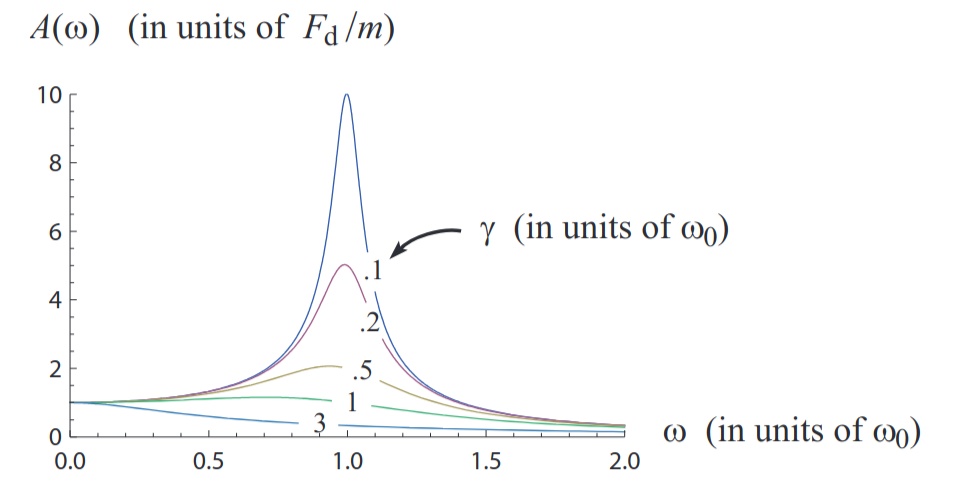
\includegraphics[width=\linewidth]{resonance_amplitude.png}
  }
  \hfill
  \subcaptionbox*{}[.48\linewidth]{
    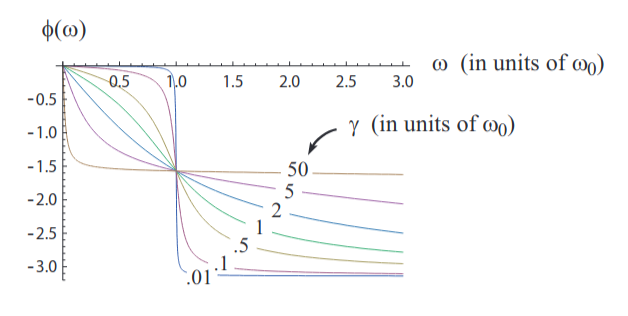
\includegraphics[width=\linewidth]{resonance_phase.png}
  }
\end{figure}

To help interpret the amplitude graph, we will introduce a new quantity: the \textbf{full width at half maximum} (FWHM; denoted by $\Gamma$). If we denote the maximum amplitude as $A_\text{peak}$, then $\Gamma$ describes the difference between the two $\omega$ values where $A = A_\text{peak}/2$. 

Assuming that $\gamma \ll \omega_0$, we have $A_\text{peak}/2 = F_d/(2\gamma m\omega_0)$. Then, if we say $\omega_{1/2}$ is the frequency where $A=A_\text{peak}/2$, 
\begin{align*}
    \frac{F_d}{2m\gamma\omega_0} &= \frac{F_d}{m}\frac{1}{\sqrt{(\omega_0^2-\omega_{1/2}^2)^2+(\gamma\omega_{1/2})^2}} \\
    4\gamma^2\omega_0^2 &= (\omega_0^2-\omega_{1/2}^2)^2+(\gamma\omega_{1/2})^2 \\
    \intertext{We can use the approximation $\omega_{1/2} \approx \omega_0$ on the $\gamma\omega_{1/2}$ term but \textbf{not} on the $\omega_0^2-\omega_{1/2}^2$ term (because the difference is so small, slight variations have a large impact). Thus,}
    4\gamma^2\omega_0^2 &\approx  (\omega_0^2-\omega_{1/2}^2)^2 + \gamma^2\omega_0^2  
\end{align*}
Or, rearranging slightly,
\begin{align*}
    (\omega_0^2-\omega_{1/2}^2)^2 &= 3\gamma^2\omega_0^2 \\
    \omega_{1/2}^2 &= \omega_0^2\pm \sqrt{3}\gamma\omega_0 \\
    \omega_{1/2} &= \omega_0\sqrt{1 \pm \sqrt{3}\frac{\gamma}{\omega_0}}
\end{align*}
Taylor expanding the square root term, we get $\sqrt{1\pm\sqrt{3}\gamma/\omega_0} \approx 1\pm \frac{\sqrt 3\gamma}{2\omega_0}$, so
\[ \omega_{1/2} = \omega_0 \pm \frac{\sqrt{3}}{2}\gamma\]
Then, the difference between the two $\omega_{1/2}$s is given by $\Gamma = \sqrt{3}\gamma$.

\section{Power}
In a driven and damped oscillator, the driving force feeds energy into the system at some points and takes energy out at others (except in the special case of resonance, where it always feeds energy in). The damping force always takes energy out. For the steady-state solution, the motion is periodic and so on average, the energy should remain constant. 

This means that the sum of the average powers from the driving force and the damping force over a complete oscillation should be zero.

For the following sections, assume the effect from the transient solution is negligible.
\subsection*{Power From the Damping Force}
Recall that the instantaneous power on an object from a force $F$ is $P =  Fv$. Therefore, 
\begin{align*}
    P_\text{damping} &= F_\text{damping}\dot x = -b\dot x^2  \\
    &= -b(-\omega A\sin(\omega t+\phi))^2 \\
    &= -b(\omega A)^2\sin^2(\omega t+\phi)
\end{align*}
The average power over a complete cycle is given by
\begin{align*}
    \langle P_\text{damping}\rangle &= \frac{1}{T}\int_0^T P_\text{damping}\dd t \\
    &= -b(\omega A)^2\pqty{\frac{1}{T}\int_0^T \sin^2(\omega t+\phi)\dd t} \\
    &= -\frac{1}{2}b(\omega A)^2
\end{align*}
Where the final equality comes from the fact that $\sin^2 \theta$, when integrated over a cycle, has an average value of $1/2$. 
\subsection*{Power From the Driving Force}
The instantaneous power from the driving force is
\begin{align*}
    P_\text{driving} &= F_\text{driving}\dot x = F_dA\cos(\omega t)\dot x \\
    &= -\omega F_dA\cos(\omega t)\sin(\omega t+\phi) \\
    &= -\omega F_dA\cos(\omega t)\pqty{\sin(\omega t)\cos(\phi) + \cos(\omega t)\sin(\phi)} \\
    &= -\omega F_dA\pqty{\cos(\phi)\sin(\omega t)\cos(\omega t) + \sin(\phi)\cos^2(\omega t)}
\end{align*}
The average value of the $\sin(\omega t)\cos(\omega t)$ term over a cycle is zero, and the average value of the $\cos^2(\omega t)$ term over a cycle is $1/2$, so
\[ \langle P_\text{driving} \rangle = -\frac{1}{2}F_dA\omega\sin\phi \]
We can rewrite $\sin\phi = -\gamma \omega mA/F_d$ (this is given without proof) to find
\[ \langle P_\text{driving}\rangle = \frac{1}2b(A\omega)^2\]
Therefore, we find $\langle P_\text{driving}\rangle + \langle P_\text{damping}\rangle = 0$, as expected. 

We will now turn our attention to $\langle P_\text{driving}\rangle$ on its own. If we plug in for $A$, we find that
\begin{align*}
    \langle P_\text{driving}\rangle &= \frac{1}{2}b\omega^2 \pqty{\frac{F_d}{m}\frac{1}{\sqrt{(\omega_0^2-\omega^2)^2+(\gamma\omega)^2}}}^2 \\
    &= \frac{\gamma mF_d^2}{2\gamma^2m^2}\frac{\gamma^2\omega^2}{(\omega_0^2-\omega^2)^2+(\gamma\omega)^2} \\
    &= \frac{F_d^2}{2\gamma m}\frac{\gamma^2\omega^2}{(\omega_0^2-\omega^2)^2+(\gamma\omega)^2}
\end{align*}
If we rewrite this as $\langle P_\text{driving}\rangle = (F_d^2/(2\gamma m)) f(\omega)$, we can plot the dimensionless quantity $f$ as a function of $\omega$. We may also plot the quantity $f/\gamma$ to see the actual average power, including the adjustment from $\gamma$.
\begin{figure}[t!]
  \subcaptionbox*{}[.48\linewidth]{
    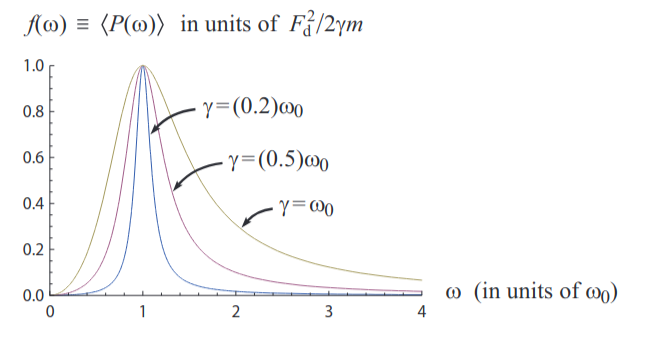
\includegraphics[width=\linewidth]{resonance_average_power_normed.png}
  }
  \hfill
  \subcaptionbox*{}[.48\linewidth]{
    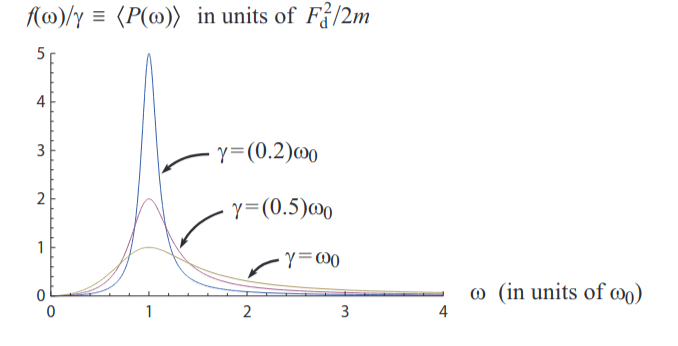
\includegraphics[width=\linewidth]{resonance_average_power_unnormed.png}
  }
\end{figure}
To find the maximum value of $f(\omega)$, we set its derivative equal to zero:
\begin{align*}
    \dv{f}{\omega} &= \frac{[(\omega_0^2-\omega^2)^2+(\gamma\omega)^2][2\gamma^2\omega] - [\gamma^2\omega^2][-4\omega(\omega_0^2-\omega^2)+2\gamma^2\omega]}{[(\omega_0-\omega^2)^2 + (\gamma\omega)^2]^2} 
\end{align*}
The denominator is never zero, so we can just set the numerator equal to zero,
\begin{align*}
    [\gamma^2\omega^2][-4\omega(\omega_0^2-\omega^2)+2\gamma^2\omega] &= [(\omega_0^2-\omega^2)^2+(\gamma\omega)^2][2\gamma^2\omega] \\
    -2\omega^2(\omega_0^2-\omega^2)+\gamma^2\omega^2 &= (\omega_0^2-\omega^2)^2 +(\gamma\omega)^2 \\
    (\omega_0^2-\omega^2)(\omega_0^2+3\omega^2) &= 0
\end{align*}
Therefore, the maximum is achieved at $\omega=\omega_0$. We also find that the maximum value of $f(\omega)$ is equal to one, so to find $\Gamma$ we set it equal to $1/2$. This means that
\[ \frac{\gamma^2\omega^2}{(\omega_0^2-\omega^2)^2+(\gamma\omega)^2} = \frac{1}{2}\]
implying that $\omega_0^2-\omega^2 = \pm \gamma\omega$. If we let $\omega_1$ be the solution given by $\omega_0^2-\omega_1^2 = \gamma\omega_1$ and $\omega_2$ be the solution given by $\omega_0^2-\omega_2^2= -\gamma\omega_w$, we take the difference to find
\begin{align*}
    \omega_2^2 - \omega_1^2 = \gamma(\omega_2+\omega_1) \implies \omega_2-\omega_1 = \gamma
\end{align*}
Therefore, the FWHM of this curve is given by $\Gamma = \gamma$. This is a nice result, and unlike the previous resonance results, holds in its exactness no matter the size of $\gamma$ (as we used no approximations to get here).

% \begin{align*}
%     \omega^2 &= \frac{2\omega_0^2+\gamma\pm \sqrt{(2\omega_0^2+\gamma^2)^2-4(\omega_0^4-4\gamma^2\omega_0^2)}}{2} \\
%     &= \omega_0^2 + \frac{\gamma^2}{2} \pm \frac{1}{2}\sqrt{4\omega_0^4+4\omega_0^2\gamma^2+\gamma^4 - 4\omega_0^4 + 16\gamma^2\omega_0^2} \\
%     &= \omega_\text{resonance}^2 \pm \frac{1}2\sqrt{20\omega_0^2\gamma^2 + \gamma^4} \\
%     &= \omega_\text{resonance}^2 \pm \frac{\gamma}{2}\sqrt{20\omega_0^2+\gamma^2}
% \end{align*}



% Consider a mass $m$ attached to a spring with spring constant $k$ that is undergoing a damping force with coefficient $b$. Now, suppose the mass has some periodic external force $F=F_D\cos\omega t$. Then, the equation of motion is given by
% \[ m\ddot x +b\dot x+k x = F_D\cos\omega t\]
% We will also write $\tilde F = F_De^{i\omega t}$, so $F_D\cos\omega t = \Re \tilde F$. We will rephrase our differential equation as
% \[ m\ddot x + b\dot x +k x = F_De^{i\omega t} \]
% Although this is slightly different, it turns out we can just take the real part at the end. Now, we guess a solution of the form
% \[ x(t) = Ae^{i(\omega t+\phi)} \]
% Notice that we have just claimed that the frequency of the motion is  the same as the frequency of the driven oscillator. In reality, there are two parts of a solution: the \textbf{transient solution}, which is determined by the initial conditions (and dies down to zero as $t$ increases; the transient solution is the solution to the homogeneous equivalent of our equation of motion), and the \textbf{steady-state solution}, which is determined by the driving force, and will persist. We claim that the frequency of the steady-state solution is the same as the frequency of the driving force
% \[ \Re x(t) = |A|\cos(\omega t+\phi)\]
% plugging this in to our differential equation,
% \[ Ae^{i\omega t}(-m\omega^2 + ib\omega + k) = F_De^{i\omega t} \]
% where $A = |A|e^{i\phi}$. Now, we can solve for $A$ to obtain
% \begin{align*}
%     A &= \frac{F_D}{-m\omega^2-ib\omega+k} \\
%     &= \frac{F_D}{m}\pqty{\frac{1}{-\omega^2+i\omega(b/m) + (k/m)}} \\
%     &= \frac{F_D}{m}\pqty{\frac{1}{(\omega_0^2-\omega^2) + i\omega\gamma}}
% \end{align*}
% We wish to remove the complex part from the denominator, so we multiply the numerator and denominator by $(\omega_0^2-\omega^2)-i\omega\gamma)$ to obtain
% \begin{align*}
% A &= \frac{F_D}{m}\pqty{\frac{(\omega_0^2-\omega^2)-i\omega\gamma}{(\omega_0^2-\omega^2)^2+\omega^2\gamma^2}}
% \end{align*}
% The magnitude of $A$ is then
% \begin{align*}
%     |A|^2 = AA^* &= \pqty{\frac{F_D}{m}}^2\pqty{\frac{(\omega_0^2-\omega^2)^2+\omega^2\gamma^2}{[(\omega_0^2-\omega^2)^2+\omega^2\gamma^2]^2}}\\
%     &= \pqty{\frac{F_D}{m}}^2\pqty{\frac{1}{(\omega_0^2-\omega^2)^2+(\omega\gamma)^2}}
% \end{align*}
% So
% \[ |A| = \frac{F_D}{m}\frac{1}{\sqrt{(\omega_0-\omega)^2+(\gamma\omega)^2}}\]
% To find the phase of $A$, we note that $\tan\phi = \Im A/\Re A$, so
% \begin{align*}
    % \tan\phi &= \frac{-\omega \gamma}{\omega_0^2-\omega^2}
% \end{align*}
% we may also use $\sin\phi = -\omega\gamma m|A|/F_D$.

% One important result is that $\phi$ is always negative--this means that the position is always lagging behind the force, which makes sense with our concept of acceleration. Further, as $\omega\to 0$, $\phi\to 0$ and as $\omega\to\infty$, $\phi\to -\pi$.

% As $\omega\to 0$, we have $|A|\to F_D/k$, so $F_D\to k|A|$. This means that the driving force balances the restoring force; $F_D + F_s = k|A| - kx$ and the system approaches a steady state. 

% Consider the power given to the system by the driving force. It is given by $P=F\dot x = F_D\cos(\omega t) \dot x$, so
% \[ P = -F_D\omega |A|\cos\omega t\sin\omega t\]
% (the $+\phi$ goes away because $\omega$ is small and so $\phi\to 0$). Then, the total work done in a period is $\int_0^T P\dd t = 0$, because the sinusoidal terms cancel each other out. Thus, on average, the driving force does no work on the system.

% When $\omega$ is very large, a very similar argument can be used to find that the driving force does very little work.

% Now, we will consider what happens when $\omega = \omega_0$. The amplitude becomes
% \[ |A| = \frac{F_D}{m}\frac{1}{\omega\gamma}\]
% We can rewrite this as
% \begin{align*}
%     |A| &= \frac{F_D}{m\omega_0^2}\frac{\omega_0}{\gamma} = \frac{F_D}{m(k/m)}\frac{\omega_0}{\gamma} \\
%     &= \frac{F_D}{k}\frac{\omega_0}{\gamma} = \frac{F_D}{k}Q
% \end{align*}
% This essentially means that if $Q$ is larger, we can get a higher resonant amplitude much easier. 

% We can additionally find that $\dd |A|^2/\dd \omega = 0$ when $\omega= \sqrt{\omega_0^2-\gamma^2/2}\approx \omega_0$ (small $\gamma$). Therefore, the amplitude is at its maximum when $\omega\approx \omega_0$.

% And the phase becomes $\phi = -\pi/2$ because $\tan\phi\to\pm \infty$. This is how we discoverer resonances in nature; by looking for a simultaneous amplitude peak and a 90 degree phase shift.

% Computing the power in this scenario, we have
% \begin{align*}
%     P = Fv &= F_D\cos(\omega t)\cdot |A|\omega \sin(\omega t +\pi/2) \\
%     &= F_D\omega|A|\cos^2(\omega t)
% \end{align*}
% This arises because the driving force and velocity are exactly in phase at the resonance, and therefore obtain peak amplitude.

% The resonant frequency is where the most efficient delivery of energy occurs. 

% We also wish to study the dissipative force at the resonant amplitude. Recall that when in resonance, 
% \[ x_s(t) = |A_s|\cos(\omega_0 t - \pi/2) = |A_s|\sin(\omega_0 t)\]
% so $v_s(t) = -|A_s|\omega_0\cos(\omega_0 t)$. Plugging this into $F_\text{drag} = -bv$, we have
% \[ F_\text{drag} = -b|A_s|\omega_0\cos(\omega_0t) = -\frac{bF_D\omega_0}{m\omega_0\gamma}\cos(\omega_0t) = -F_D\cos(\omega_0t)\]
% This essentially tells us that at the peak of the resonance, the driving force and resistant force cancel each other out.

% We will define a new quantity known as the \textbf{full width half maximum} (FWHM), denoted by $\Gamma$, which tells us the distance between the two points on a graph of $|A|$ vs $\omega$ where $|A| = |A|_\text{peak}/2$. In other words, it is the distance between $\omega_1$ and $\omega_2$ where
% \[ |A|_{\omega_1} = |A|_{\omega_2} = \frac{F_D}{2m}\frac{1}{\gamma\omega}\]
% Therefore, if $\omega'$ is either $\omega_1$ or $\omega_2$,
% \begin{align*}
%     \frac{F_D}{m}\frac{1}{\sqrt{(\omega_0^2-\omega'^2)^2+(\gamma\omega')^2}} &= \frac{F_D}{m}\frac{1}{2\gamma\omega} \\
%     (\omega_0^2-\omega'^2)^2 + (\gamma\omega')^2 &= 4\gamma^2\omega_0^2 \\
%     \omega'^4 - (2\omega_0^2+\gamma^2)\omega'^2 + \omega_0^4(1-4\gamma^2) &= 0
% \end{align*}
% So FWHM $ = \sqrt{3} \gamma$.

% \subsection*{Including the Transient Solution}
% Previously, we made the claim that the steady solution dominates as $t\to\infty$. Now, we justify that claim.

% First, suppose the transient solution is $x_\text{tr}(t)$ and the steady solution is $x_\text{s}(t)$. The most general form of $x(t)$ is
% \begin{align*}
%     x(t) &= x_\text{tr} + x_\text{s} \\
%     &= |A_\text{tr}|e^{-\gamma t/2}\cos(\omega't+\phi') + |A_\text{s}|\cos(\omega t + \phi)
% \end{align*}
% With the initial condition $x(0)=0$ and $x'(0)=0$, we have $\phi' = -\pi/2$ and $|A_\text{tr}| = |A_\text{s}|$. Additionally, for small $\gamma$ we have $\omega' \approx \omega_0$, and at resonance $\omega \approx \omega_0$. Then, $x(t)$ becomes
% \[ x(t) = |A_\text{s}|(1-e^{-\gamma t/2})\sin(\omega t)\]
% So as $t$ increases, $x(t)\to x_\text{s}(t)$. The amount of time it takes for the transient solution to die down is proportional to $\tau = 1/\gamma$. 
% \subsection*{Power Delivery (General Frequency)}
% Assuming the transient solution is sufficiently small, the instantaneous power from the driving force is given by $P_D = (F_D\cos\omega t)(-|A|\omega\sin(\omega  t + \phi))$. The average power over a period of oscillation is given by
% \begin{align*}
%     \langle P_D\rangle &= \frac{1}{T}\int_0^T P\dd t \\
%     &= -\frac{F_D\omega|A|}{T}\int_0^T \cos(\omega t)\sin(\omega t +\phi) \dd t \\ 
%     &= -\frac{F_D\omega|A|}{T}\int_0^T \cos(\omega t)\pqty{\sin\omega t \cos\phi + \cos\omega t\sin\phi} \dd t \\
%     &= -\frac{F_D\omega|A|\cos\phi}{T}\int_0^T \cos\omega t\sin\omega t \dd t - \frac{F_D\omega |A|\sin\phi}{T}\int_0^T \cos^2\omega t\dd t
%     \intertext{The left term goes to zero, so }
%     \langle P_D \rangle &= -\frac{F_D\omega|A|\sin\phi}{T}\int_0^T \cos^2\omega t \dd t \\
%     &= -\frac{F_D\omega |A|\sin\phi}{2} = -\frac{F_D\omega|A|(-\omega\gamma m|A|)}{2F_D} = \frac{1}{2}b\omega^2|A|^2 
% \end{align*}
% The instantaneous power from the dissipating force is given by $P_R = -bv^2 = -b\omega^2|A|^2\sin^2(\omega t+\phi)$. So the average power from the dissipating force over a period of oscillation is
% \begin{align*}
%     \langle P_R\rangle &= \frac{1}{T}\int_0^T -b\omega^2|A|^2\sin^2(\omega t+\phi)\dd t \\
%     &= -\frac{1}{2}b\omega^2|A|^2
% \end{align*}
% So the total average power over an oscillation is $\langle P\rangle = \langle P_R\rangle + \langle P_D\rangle = 0$. This means that the energy of a steady driven harmonic oscillator is constant. Also note that these results apply at any frequency, not just in resonance. 

% Although the driving power will always cancel with the resistive power, the magnitude of the power input into the system (by the driving force) is given by
% \begin{align*}
%     \langle P_D\rangle &= \frac{F_D^2}{2m\gamma}\frac{\gamma^2\omega^2}{(\omega_0^2-\omega^2)^2+(\gamma\omega)^2} 
% \end{align*}
% which tells us that the power peaks at the resonance $\omega=\omega_0$, with a value of
% \[ \langle P_D\rangle_\text{max} = \frac{F_D^2}{2m\gamma} \]
% We also find that the FWHM of this curve is exactly $\Gamma = \gamma$. Therefore, we have $\Gamma\tau = 1$, which is one of the critical universal properties of resonant motion. 
